\documentclass[margin=10pt]{standalone}
\usepackage{color,xcolor}

\usepackage[utf8]{inputenc} 
\usepackage{pgf-umlsd}
\usetikzlibrary{patterns}



\usepackage{ifluatex}% Test
\usepackage{amsmath}  %% muss vor fontspec geladen werden

\ifluatex
\usepackage{fontspec}% Vektorschrift
\usepackage{unicode-math}% Mathematikschrift
\usepackage{babel}
\usepackage[german=guillemets]{csquotes}
\usepackage{microtype} % optischer Randausgleich etc.

%\setmathfont[Scale=0.9]{texgyrepagella-math.otf}
%\setmathfont{XITS Math}
\newfontface\Erna[%
Scale=MatchUppercase]{Arial}
\else
\usepackage[T1]{fontenc}%Schriftkodierung
\usepackage{kpfonts}%Kepler Fonts mit mathe
\usepackage[utf8]{inputenc}% Eingabekodierung
\fi





\usepackage{xspace}
\usepackage{tcolorbox}
\usepackage{caption}
\usepackage[labelformat=simple]{subcaption}
\renewcommand\thesubfigure{(\alph{subfigure})}
\usepackage{listings}
\usepackage{siunitx}
\usepackage{todonotes}
\usepackage[outdir=./]{epstopdf}
\usepackage{graphicx}
\usepackage{nbaseprt}
\usepackage{colortbl}
\usepackage{setspace}
\usepackage{tikz-uml}






\usepackage{relsize}
\usepackage{tkz-euclide}
\usepackage{pgfplots}
\usepackage{multirow}
\usepackage{pgfplotstable} % Generates table from .csv
\usepackage{array}
\usepackage{makecell}
\usepackage[ruled, lined, linesnumbered, commentsnumbered, longend]{algorithm2e}
\usepackage[edges]{forest}
\usepackage{listings}
\usepackage{xcolor}
\usepackage{capt-of}
\usepackage{enumitem}


\makeatletter




\newcommand{\at}{\makeatletter @\makeatother}









\usetikzlibrary{%
	arrows,%
	calc,
	shapes,
	arrows,
	shapes.misc,% wg. rounded rectangle
	shapes.arrows,%
	chains,%
	matrix,%
	positioning,% wg. " of "
	scopes,%
	decorations,% /pgf/decoration/random steps | erste Graphik
	shadows,%
	3d,%
	patterns,%
	patterns.meta,%
	automata,%
	backgrounds,%
	intersections,%
	tikzmark,%
	positioning,%
	angles,%
	quotes,%
	calc,
	fit
}



\tikzset{
	box/.style = {
	fill = black!5,
	line width=1mm,
	inner sep=1.5em,
	rounded corners= 1em,
	draw=black,
	fill opacity=0.5,
	draw opacity = 0.7	
	}
}

\tikzset{% UML2 Activity Diagram Styles
	caption/.style    = {node distance=1em},
	process/.style    = {fill=black!5,draw, thick, rounded corners=0.8em, minimum height = 3em,
		minimum width = 5em, align=center, inner sep=1em,node distance=1em},
	object/.style    = {fill=black!5,draw, thick, rectangle, minimum height = 3em,
		minimum width = 3em, align=center, inner sep=1em,node distance=1em},
	pin/.style    = {fill=black!5,draw, thick, rectangle, minimum height = 0.6em,
		minimum width = 0.6em, node distance=-1pt, inner sep=0,font=\relsize{-3.5}},
	start/.style      = {fill=black,draw,circle,node distance=1em}, 
	group/.style      = {color=black,thin,rounded corners=0.8em, rectangle,fill = black!5}, 
	groupCaption/.style      = {above=0.2cm,very thick,right=0.2cm, fill = white,draw = black,font = \scshape}, 
	input/.style    = {coordinate,node distance=1.5em}, 
	output/.style   = {coordinate,node distance=1.5em}, 
	between/.style args={#1 and #2}{ % http://tex.stackexchange.com/a/138828/15602
		at = ($(#1)!0.5!(#2)$)
	},
	notefield/.style    = {fill=green!5,draw, thick, minimum height = 3em,
		minimum width = 3em, align=left, inner sep=0.5em,node distance=3em,,text width=4cm},
	loop/.style = { rounded corners=0.8em,dashed,rectangle split, rectangle split,
		rectangle split parts=3, very thick,draw=black,  align=center,minimum height = 4cm,rectangle split part align={center, left, left}},
	fitting node/.style={
		inner sep=0pt,
		fill=none,
		draw=none,
		reset transform,
		fit={(\pgf@pathminx,\pgf@pathminy) (\pgf@pathmaxx,\pgf@pathmaxy)}
	},
	reset transform/.code={\pgftransformreset}
	
}



\tikzset{
	base/.style    = {
		rectangle,
		draw,
		anchor=west,
		minimum height=0.8cm,
		minimum width=1.6cm,
		fill=white,
		drop shadow={opacity=0.5,fill=black},
		node distance = 7cm
	},%
	node/.style = {
		base,
		fill = \nodecol,
	},%
	ecs/.style = {
		base,
		fill=\ecsscol
	},%
	active/.style = {
		rectangle,
		draw,
		minimum width = 0.2cm,
		minimum height=1cm,
		fill = gray!20,
		node distance = 1mm and 1cm
	},%
	lifeline/.style ={
		line width=0.3mm,
		-,
		color = black,
		line cap = round,
		dash pattern=on 0pt off 2.5pt
	},%
	secop/.style ={
		line width=0.5mm,
		color = black
	},%
	synchron/.style ={
		->,
		>=triangle 60
	},%
	asynchron/.style ={
		->,	
		>=angle 60
	},%
	syncreturn/.style ={
		->,	
		dashed,
		>=angle 60
	},%
	mess/.style ={
		->,
		>=angle 60
	},%
	messtext/.style ={
		font= \scriptsize\ttfamily,
		midway,
		above,
		sloped,
		align = center,
		text width = 7.5cm 
	},%
	blockstyle/.style={
	anchor = north west,
	font =\ttfamily
	}
}

\tikzset{
	statbar/.style    = {
		font = \scriptsize,
		rectangle,
		draw,
		thin,
		minimum width=0.4cm,
		node distance = 0cm,
		opacity = 0.4,
		inner sep = 2pt
	},%
	statidle/.style    = {
		statbar,
		fill = idle,
		draw = idle
	},%
	statbusy/.style    = {
		statbar,
		fill = busy,
		draw = busy
	},%
	statundefined/.style    = {
		statbar,
		pattern=north west lines,
		pattern color=gray,
		draw = gray
	}%
}


\definecolor{devicecol}{HTML}{fc8d59}
\definecolor{signalcol}{HTML}{91bfdb}
\definecolor{signalxcol}{HTML}{ffffbf}

\def\devcol{devicecol!60}
\def\sigcol{signalcol!60}
\def\sigxcol{signalxcol!60}


\newcommand{\drawll}[2]{
	\draw[lifeline] (#1) -- ([yshift=- #2] #1);
}


\newcommand{\makeGroup}[6]{
	\draw [group,fill= #6](#2-0.5,#3+1.5-#5)rectangle(#2+#4+0.5,#3+1.5);
	\node at (#2,#3+1.5) [groupCaption] {#1};
}



%### DEFINITIONS


%### COLORS

% SECoP Classes
\definecolor{ecscolor}{HTML}{648FFF}
\definecolor{nodecolor}{HTML}{DC267F}
\definecolor{modulecolor}{HTML}{844D30}
\definecolor{accessiblecolor}{HTML}{785EF0}
\definecolor{properycolor}{HTML}{FFB000}

% SECoP Protocol Message
\definecolor{SECoPProtocol}{HTML}{FE6100}

% Hardware Colors
\definecolor{hardwarecol}{HTML}{054A16}




\newcommand{\propcol}{signalcol!60}
\newcommand{\nodecol}{devicecol!60}
\newcommand{\modcol}{devicecol!60}
\newcommand{\accesscol}{signalcol!60}
\newcommand{\ecsscol}{ecscolor!50}

% STATUS Code Colors
\definecolor{disabled}{HTML}{b3b3b3}
\definecolor{idle}{HTML}{008450}
\definecolor{warn}{HTML}{db7b2b}
\definecolor{busy}{HTML}{EFB700}
\definecolor{error}{HTML}{B81D13}












%##########################
% DEFINES

\def\lllength{9.75cm}



\pgfdeclarelayer{bbackground layer}
\pgfdeclarelayer{background layer}
\pgfdeclarelayer{foreground layer}
\pgfsetlayers{bbackground layer,background layer,main,foreground layer}

\begin{document}
	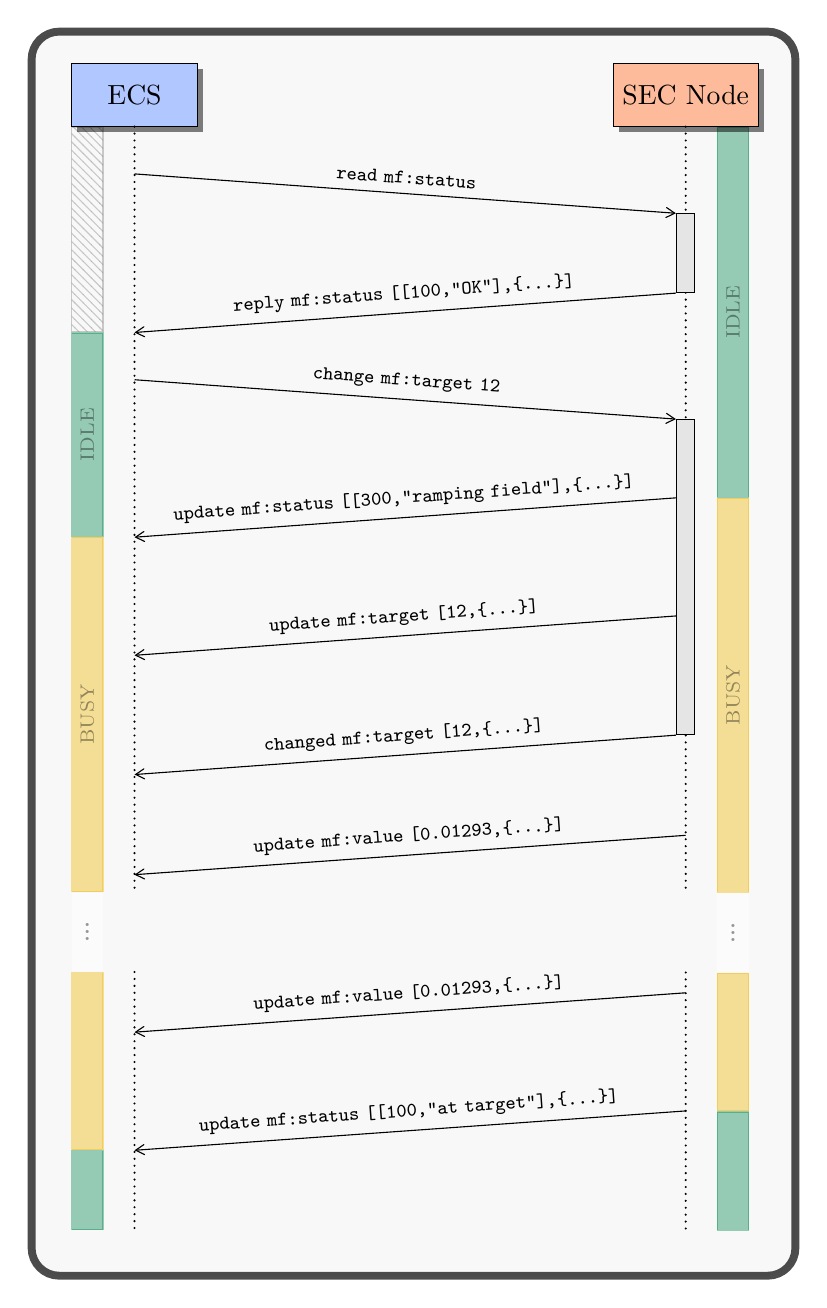
\begin{tikzpicture}
		
		
		
		\draw
		node[ecs](ecs){ECS}
		node[node,right  of =  ecs](node){SEC Node}	
		;
		
		\drawll{ecs.south}{\lllength}
		\drawll{node.south}{\lllength}
		
		
		\coordinate(llecs)  at (ecs.south);
		\coordinate(llnode) at (node.south);
		
		
		
		\draw	
		
		node[active,below = of node, yshift = -1cm] (readstat){}
		
		node[active,below = of readstat,minimum height = 4cm, yshift = -1.5cm] (changetarget){}
		
		
		
		;
		
		
		%##### Read Status
		\draw[mess] let \p1= (readstat.north west),
		\p2= (ecs.south) in
		(\x2,\y1 + 0.5cm) -- node [messtext] {read mf:status}(\p1);
		
		
		
		\draw[mess] let \p1= (readstat.south west), 
		\p2= (ecs.south) in
		(\p1) -- node [messtext]{reply mf:status [[100,"OK"],\{...\}]}(\x2,\y1 - 0.5cm);
		
		%##### change
		
		\draw[mess] let \p1= (changetarget.north west),
		\p2= (ecs.south) in
		(\x2,\y1 + 0.5cm) -- node [messtext] {change mf:target 12}(\p1);
		
		
		
		\draw[mess] let \p1= (changetarget.south west), 
		\p2= (ecs.south) in
		(\p1) -- node [messtext]{changed mf:target [12,\{...\}]}(\x2,\y1 - 0.5cm);
		
		%#### Side Effects
		%< update mf:status [[300,"ramping field"],{...}]
		\draw[mess] let %
			\p1= (changetarget.north west), 
			\p2= (ecs.south) in
		([yshift = -1cm]\p1) -- node [messtext]{update mf:status [[300,"ramping field"],\{...\}]}([yshift = -1cm]\x2,\y1 - 0.5cm);
		
		
		%< update mf:target [12,{...}]
		\draw[mess] let %
			\p1= (changetarget.north west), 
			\p2= (ecs.south) in
		([yshift = -2.5cm]\p1) -- node [messtext]{update mf:target [12,\{...\}]}([yshift = -2.5cm]\x2,\y1 - 0.5cm);
		
		


		
		%#### post change updates
		%< update mf:value [0.01293,{...}]
			
		\draw[mess] let %
			\p1= (node.south), 
			\p2= (ecs.south) in
		([yshift = -9cm]\p1) -- node [messtext]{update mf:value [0.01293,\{...\}]}([yshift = -9cm]\x2,\y2 - 0.5cm);
		
			%### reached target
	% update mf:value [12.01194,{...}]
	
	\draw[mess] let %
	\p1= (node.south), 
	\p2= (ecs.south) in
	([yshift = -11cm]\p1) -- node [messtext]{update mf:value [0.01293,\{...\}]}([yshift = -11cm]\x2,\y2 - 0.5cm);
	
	% update mf:status [[100,"at target"],{...}]		
	
	\draw[mess] let %
	\p1= (node.south), 
	\p2= (ecs.south) in
	([yshift = -12.5cm]\p1) -- node [messtext]{update mf:status [[100,"at target"],\{...\}]	}([yshift = -12.5cm]\x2,\y2 - 0.5cm);
	
	
	\begin{pgfonlayer}{background layer}
		
		
		
		\draw
		
		% ECS Status Bar		
		node[statundefined,below = of ecs.south,xshift = -.6cm,minimum height = 2.6cm] (ecs_undefined){\rotatebox{90}{}}
		node[statidle,below = of ecs_undefined,minimum height = 2.58cm] (ecs_idle){\rotatebox{90}{IDLE}}
		node[statbusy,below = of ecs_idle,minimum height = 4.5cm] (ecs_busy){\rotatebox{90}{BUSY}}
		node[statbusy,draw = none,fill = white,below = of ecs_busy,minimum height = 1cm] (ecs_busy_dot){\rotatebox{90}{\textbf{...}}}
		node[statbusy,below = of ecs_busy_dot,minimum height = 2.25cm] (ecs_busy_cont){}
		node[statidle,below = of ecs_busy_cont,minimum height = 1cm] (ecs_idle_at_target){}
		
		% Node Status Bar
		node[statidle,below = of node.south,xshift = 0.6cm,minimum height = 4.7cm] (node_idle){\rotatebox{90}{IDLE}}
		node[statbusy,below = of node_idle,minimum height = 5cm] (node_busy){\rotatebox{90}{BUSY}}
		node[statbusy,draw = none,fill = white,below = of node_busy,minimum height = 1cm] (node_busy_dot){\rotatebox{90}{\textbf{...}}}
		node[statbusy,below = of node_busy_dot,minimum height = 1.75cm] (node_busy_cont){}
		node[statidle,below = of node_busy_cont,minimum height = 1.5cm] (node_idle_at_target){}
		
		;
		\end{pgfonlayer}

		\draw[lifeline] let 
		\p1= (node_busy_cont.north),
		\p2= (node.south),
		\p3= (node_idle_at_target.south) in
		(\x2,\y1) -- (\x2,\y3);
		
		\draw[lifeline] let 
		\p1= (ecs_busy_cont.north),
		\p2= (ecs.south),
		\p3= (ecs_idle_at_target.south) in
		(\x2,\y1) -- (\x2,\y3);
		
		\begin{pgfonlayer}{bbackground layer}
			\draw [box]	(-0.5,0.8)rectangle(9.2,-15);
		\end{pgfonlayer}	
		
		
	\end{tikzpicture}
	
	
	
	
\end{document}